\chapter{Results\label{cha:chapter6}}
\section{Data Acquisition}
The data acquisition was performed with 27 subjects in total, 12 (44\%) females and 15 (56\%) males. Participants had an average age of 26.4 years (17, 53, 6.39) and all 27 were right-handed (100\%). 19 (70\%) were students, 8 (30\%) had other occupations. All 27 (100\%) were right handed.
18 (66\%) subjects stated that their most used input modality is the their thumb while 4 (14\%) preferred using their index finger and 5(18\%) use both thumbs during interactions.\\

\begin{figure}[h!]
  \centering
  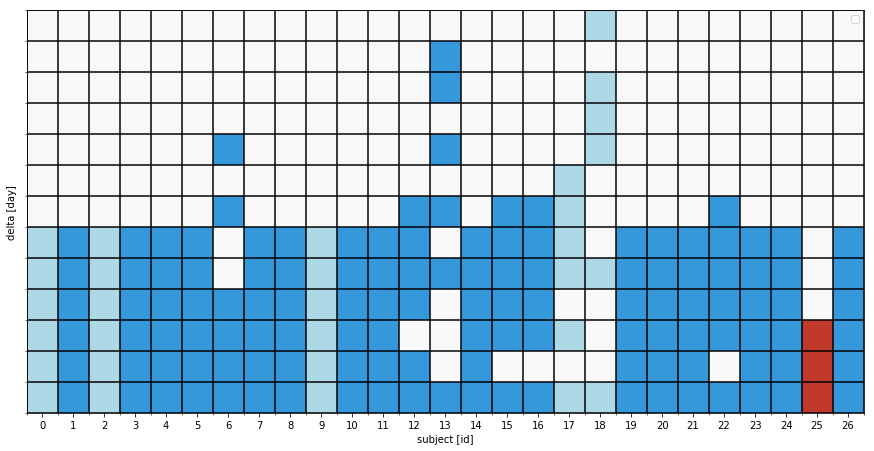
\includegraphics[width=1\textwidth]{participation_push.png}
  \caption{The figure shows on which days the participants took part in the field study. Light blue subjects which did not receive push notifications while subjects with dark blue marks had received push notifications. Red rectangles indicates a dropped out subject.} \label{fig:participation}
\end{figure}

In regards to the participation during the study, 26 subjects managed to finish all laboratory and field study trials while 1 subject dropped out in the field study. Figure \ref{fig:participation} shows on which day individual participants performed trails. 4 participants did not accept push notification and were therefore not reminded on a daily basis.

In total over 46.000 taps were generated in the whole data acquisition phase. To be more precise, approx. 25.000 taps were collected on the 5x4 grid, over 15.000 taps on the 4x3 grid and more than 5.000 taps on the 2x2 grid.

The devices used to obtain the tap information were 12 (45\%) Apple iPhone 6s, 10 (37\%) iPhone 6 and the least common device was the iPhone 7 with 5 (18\%).

\section{Lab vs. Field}
\subsection{Within subject accuracties}
\subsection{Device accuracies}
\subsection{One model}

\section{Global Model}
\subsection{Within subject accuracies}
\subsection{Device accuracies}
\subsection{One model}

\section{Discussion}
